\section{The BASE Architecture}
\label{sec:architecture}

We designed BASE to directly address the integration barriers identified in Section~\ref{sec:sensor_limitations}. It eliminates type-safety violations, resolves broken state management by moving sequencing into the kernel, and repairs leaky abstractions by isolating all vendor-specific protocol details. By integrating these solutions as a dedicated RTOS subsystem, BASE enforces secure, deterministic behavior by default.

\subsection{Three-Plane Architecture}

BASE separates concerns across three layers (Figure~\ref{fig:architecture}). The Application Plane provides unified enrollment and matching interfaces via standard RTOS system calls. The Subsystem Contract Plane normalizes hardware capabilities, enforces type safety, and abstracts protocol-specific details. The Driver Implementation Plane isolates all vendor-specific UART/SPI protocols and sensor state. No layer reaches past its boundary.

\begin{figure*}
    \centering
    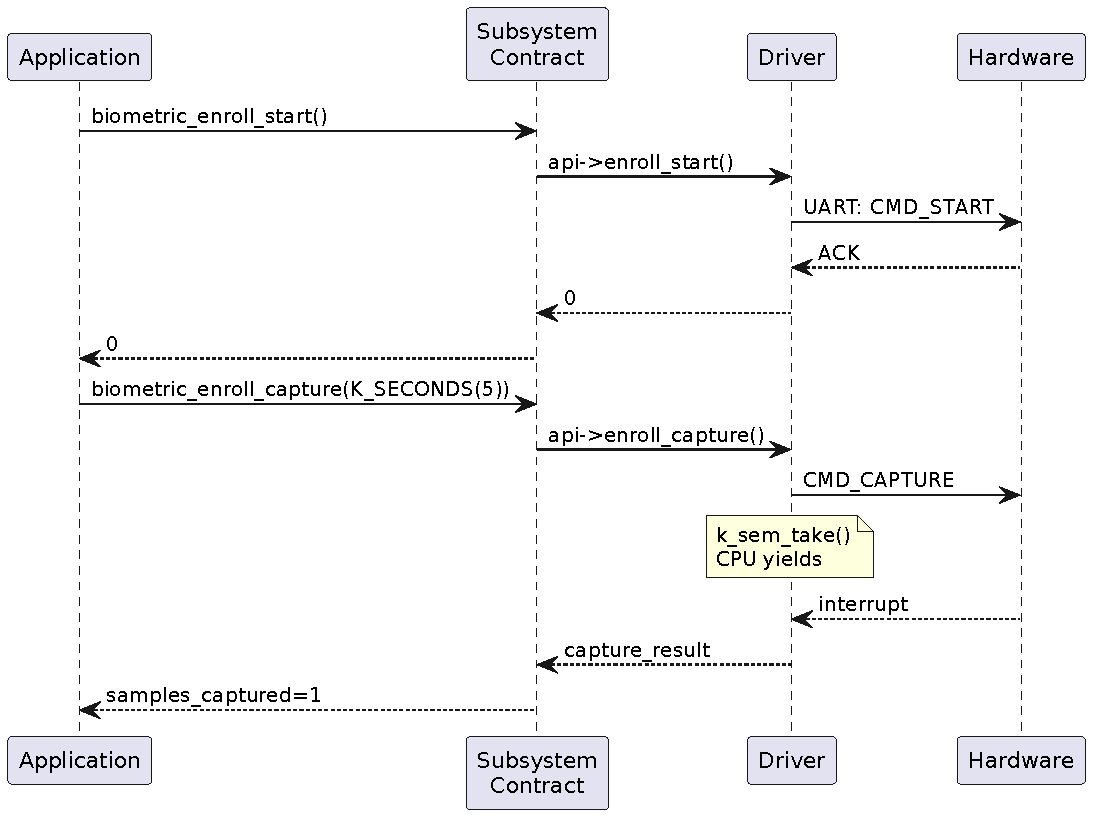
\includegraphics[width=\textwidth]{figs/fig_architecture.pdf}
    \caption{Three-plane architecture of BASE. The contract plane dispatches to three driver families spanning contact fingerprint (ZFM-X0, GT-5X) and camera-based multi-modal sensing (AI10). No layer reaches past its boundary.}
    \label{fig:architecture}
\end{figure*}

The Application Plane provides unified enrollment, matching, and template management interfaces. Applications never access hardware drivers directly. All public functions are defined via standard RTOS system calls (e.g., Zephyr's \texttt{\_\_syscall} annotation, which generates kernel-mode dispatch for each entry point), allowing the driver to run in privileged mode while the application runs in userspace. On POSIX-compliant systems such as NuttX, the same boundary is enforced via VFS \texttt{ioctl()} calls; on capability-based systems such as TockOS, via capsule syscalls. This protects the biometric state machine from application-level crashes or memory corruption. Errors are indicated by standard POSIX error codes (i.e., EBUSY, EINVAL).

The Subsystem Contract Plane defines the \\ \texttt{biometric\_driver\_api} structure that biometric drivers are required to implement. This layer normalizes different hardware capabilities into standardized attribute enumerations. It also abstracts away protocol-specific endianness. Applications work without the knowledge of whether a sensor communicates in Big Endian (ZFM-70) or Little Endian (GT-521F32).

The Driver Implementation Plane consists of hardware drivers that comply with the requirements of the Contract Plane. These drivers handle the low-level communication protocols (e.g., UART packet framing, checksum calculation) and manage the sensor's physical state. By isolating these details at the bottom of the stack, BASE ensures that protocol-level changes such as switching from a packet-based ZFM sensor to a command-based GT-5X sensor remain transparent to the higher layers. It is also possible to integrate Trusted Execution Environment (TEE), where matching logic can be further offloaded to secure zones like ARM TrustZone.

\subsection{API Specification}

\subsubsection{Core Data Types}

We defined five core types based on biometric concerns: capabilities, match outcomes, enrollment progress, policy configuration, and on-device user metadata. This allowed us to replace the legacy behavior of forcing user IDs, template count, and score into \texttt{sensor\_value} fields (Table~\ref{tab:data_types}). This is the type safety that the generic sensor API cannot provide.

\begin{table}
\caption{BASE Core Data Types}
\label{tab:data_types}
\centering
\renewcommand{\arraystretch}{1.4}
\setlength{\tabcolsep}{5pt}
\begin{tabularx}{\columnwidth}{|l|X|}
\hline
\textbf{Type} & \textbf{Purpose} \\
\hline
\texttt{biometric\_capabilities} & Hardware features: \texttt{supported\_modalities} bitmask (multi-modal), max templates, samples required, storage modes \\
\hline
\texttt{biometric\_match\_result} & Match outcome: confidence, template ID, quality (0--100), \texttt{modality} field identifying which sensing modality produced the result \\
\hline
\texttt{biometric\_capture\_result} & Enrollment progress: samples captured/required, quality, assigned template ID \\
\hline
\texttt{biometric\_attribute} & Config: match thresholds, security levels, timeouts, duplicate enrollment policy \\
\hline
\texttt{biometric\_user\_info} & On-device user metadata: name string, privilege level \\
\hline
\end{tabularx}
\end{table}

\subsubsection{Enrollment and Match APIs}
Enrollment abstracts the varying sample counts across hardware (e.g., 2 for ZFM, 3 for GT-5X, 1 for AI10). Applications repeatedly call \texttt{biometric\_enroll\_capture()} until \texttt{samples\_required} is met, then call \texttt{biometric\_enroll\_finalize()}. Similarly, the Match API hides hardware-specific search optimizations behind a unified \texttt{biometric\_match()} interface that supports both 1:1 verification and 1:N identification.

\subsubsection{API Correctness Contracts}

We specify the behavioral obligations of BASE drivers using Hoare triple notation $\{P\}\;C\;\{Q\}$, where $P$ is the precondition and $Q$ the postcondition for operation $C$. $\mathtt{stored}(\mathit{id})$ denotes template $\mathit{id}$ is persistently committed; $\mathtt{exists}(\mathit{dev},\mathit{id})$ denotes it is present; $\mathrm{DB}$ is the set of enrolled templates.

\paragraph{Enrollment start:}
\begin{multline}
  \{\mathrm{state} = q_{\mathrm{idle}}\}\;\;
  \mathtt{enroll\_start}(\mathit{dev},\,\mathit{id})\;\; \\
  \{\mathrm{state} = q_{\mathrm{w},1} \;\wedge\; \mathtt{enrolled\_id} = \mathit{id}\}
\end{multline}

\paragraph{Sample capture:} For $1 \le k \le N$, with $\sigma$
the outcome symbol (\texttt{capture\_ok} or \texttt{capture\_fail}) corresponding to the return value:
\begin{multline}
  \{\mathrm{state} = q_{\mathrm{w},k}\}\;\;
  \mathtt{enroll\_capture}(\mathit{dev},\,t,\,\&r)\\
  \{\mathrm{state} = \delta(q_{\mathrm{w},k},\,\sigma)\}
\end{multline}

\paragraph{Template finalization:}
Here $\mathit{id}$ is the logical variable bound by the preceding $\mathtt{enroll\_start}(\mathit{dev},\,\mathit{id})$ call.
\begin{multline}
  \{\mathrm{state} = q_{\mathrm{ready}}
   \;\wedge\; \mathtt{enrolled\_id} = \mathit{id}\}\;\; \\
  \mathtt{enroll\_finalize}(\mathit{dev})\\
  \{\mathrm{state} = q_{\mathrm{idle}}
   \;\wedge\; \mathtt{stored}(\mathit{id})\}
\end{multline}

\paragraph{Match non-interference.}
\begin{multline}
  \{\mathrm{DB} = \mathrm{DB}_0\}\;\;
  \mathtt{match}(\mathit{dev},\,\mathit{mode},\,\mathit{id},\,t,\,\&r)\\
  \{\mathrm{DB} = \mathrm{DB}_0\}
\end{multline}

\paragraph{Template deletion.}
\begin{multline}
  \{\mathtt{exists}(\mathit{dev},\,\mathit{id})\}\;\;
  \mathtt{template\_delete}(\mathit{dev},\,\mathit{id})\;\; \\
  \{\neg\,\mathtt{exists}(\mathit{dev},\,\mathit{id})\}
\end{multline}


\subsubsection{Auxiliary Match Output}
Sensor-specific auxiliary output, such as liveness score blobs or custom data, would either pollute \\ \texttt{biometric\_match\_result} with union fields, breaking type safety, or require sensor-specific calls, breaking the abstraction. \texttt{biometric\_match\_get\_data()} resolves this: a standardized optional side-channel, null-guarded, with a defined retrieval window (must be called before the next match operation). Rich sensor output flows through a typed buffer without contaminating the universal result structure.

\subsubsection{Portable Security Configuration}
Security parameters (Table~\ref{tab:attributes}) map normalized 0--100/1--10 ranges to hardware-specific values via \texttt{biometric\_attr\_set()}. This enables zero-code-change policy portability, allowing seamless hardware swapping without altering application compliance logic.

\begin{table}
\caption{Security Configuration Attributes}
\label{tab:attributes}
\centering
\renewcommand{\arraystretch}{1.4}
\setlength{\tabcolsep}{4pt}
\begin{tabularx}{\columnwidth}{|l|c|X|}
\hline
\textbf{Attribute} & \textbf{Range} & \textbf{Function} \\
\hline
\texttt{MATCH\_THRESHOLD} & 0--100 & Min similarity score (\%) \\
\hline
\texttt{SECURITY\_LEVEL} & 1--10 & FAR (False Accept Rate) control \\
\hline
\texttt{ENROLL\_QUALITY} & 0--100 & Min image quality \\
\hline
\texttt{TIMEOUT\_MS} & 0--3.6M & Max operation timeout (ms) \\
\hline
\texttt{ANTI\_SPOOF} & 1--10 & Liveness detection sensitivity \\
\hline
\texttt{IMAGE\_QUALITY} & read-only & Last captured sample quality score \\
\hline
\texttt{DUPLICATE\_POLICY} & 0--1 & Reject (0) or allow (1) duplicate enrollments \\
\hline
\end{tabularx}
\end{table}

A sensor supporting 1--5 security levels maps the subsystem's 1--10 scale via \texttt{hw\_level = CLAMP((val+1)/2, 1, 5)}. An application that sets 80\% match threshold and security level 8 gets those exact values regardless of which sensor is on the board. The hardware can be easily swapped with no change in the policy. This increases accessibility and portability in security-critical deployments like payment terminals, medical device access control, industrial safety interlocks etc. It also supports compliance with NIST SP 800-63B \cite{nist_800_63b}, which requires specific False Accept Rates based on the authentication assurance level. Auditors can inspect devicetree bindings or application configuration to verify compliance without looking at the driver internals. For hardware-specific parameters, the enum reserves \texttt{BIOMETRIC\_ATTR\_PRIV\_START} and above for driver-private attributes, accessible through the same \texttt{biometric\_attr\_set()} interface without requiring sensor-specific headers in application code. The attribute-based security model aligns with contemporary recommendations for IoT device authentication\cite{wu2023attacks,sicari2015security}.

\begin{figure*}
    \centering
    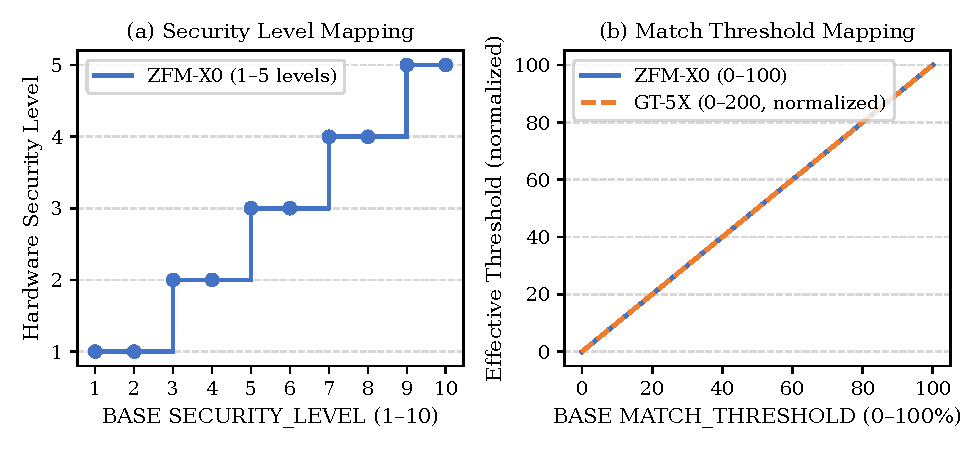
\includegraphics[width=\textwidth]{figs/fig_normalization.pdf}
    \caption{Attribute normalization mapping curves.}
    \label{fig:normalization}
\end{figure*}

\subsection{Enrollment State Machine}

To guarantee deterministic behavior, BASE mandates a strict enrollment state machine via the MUST contract. We formalize this as a Deterministic Finite Automaton $\mathcal{A} = (Q, \Sigma, \delta, q_0, F)$. \\

\noindent\textbf{States.} For a sensor requiring $N$ samples:
\begin{equation}
  Q = \{q_{\mathrm{idle}},\;
        q_{\mathrm{w},1},\; \ldots,\; q_{\mathrm{w},N},\;
        q_{\mathrm{ready}}\}
  \label{eq:states}
\end{equation}
$q_{\mathrm{idle}}$: subsystem inactive. $q_{\mathrm{w},k}$: enrollment active, $k{-}1$ samples captured, awaiting the $k$-th. $q_{\mathrm{ready}}$: all $N$ samples captured; driver authorized to commit the template. \\

\noindent\textbf{Input alphabet:}
\begin{multline}
  \Sigma = \{\mathtt{start},\;
             \mathtt{capture\_ok},\;
             \mathtt{capture\_fail},\; \\
             \mathtt{finalize},\;
             \mathtt{abort}\}
  \label{eq:alphabet}
\end{multline}

\noindent\textbf{Transition function:}
\begin{align}
  \delta(q_{\mathrm{idle}},\; \mathtt{start})
    &= q_{\mathrm{w},1}
    \label{eq:d_start}\\
  \delta(q_{\mathrm{w},k},\; \mathtt{capture\_ok})
    &= q_{\mathrm{w},k+1},
    \quad 1 \le k < N
    \label{eq:d_ok}\\
  \delta(q_{\mathrm{w},N},\; \mathtt{capture\_ok})
    &= q_{\mathrm{ready}}
    \label{eq:d_final}\\
  \delta(q_{\mathrm{w},k},\; \mathtt{capture\_fail})
    &= q_{\mathrm{w},k},
    \quad 1 \le k \le N
    \label{eq:d_fail}\\
  \delta(q_{\mathrm{ready}},\; \mathtt{finalize})
    &= q_{\mathrm{idle}}
    \label{eq:d_finalize}\\
  \delta(q,\; \mathtt{abort})
    &= q_{\mathrm{idle}},
    \quad \forall\, q \in Q \setminus \{q_{\mathrm{idle}}\}
    \label{eq:d_abort}
\end{align}

Any $(q, \sigma)$ pair not listed above leaves the state unchanged; the API call returns \texttt{-EINVAL}, with the exception that $\delta(q_{\mathrm{idle}},\,\mathtt{abort})$ returns \texttt{-EALREADY}, distinguishing the ``already idle'' condition from a malformed call. Initial state $q_0 = q_{\mathrm{idle}}$; accepting state $F = \{q_{\mathrm{ready}}\}$. Figure~\ref{fig:fsm} illustrates $\mathcal{A}$ for $N = 2$.

\begin{proposition}[No Partial Template Storage]
\label{prop:safety}
For any execution trace $\tau \in \Sigma^*$, a template is committed to persistent storage only after exactly $N$ $\mathtt{capture\_ok}$ events following the most recent $\mathtt{start}$ event.
\end{proposition}

\begin{proof}
Template storage is triggered exclusively by \\ $\delta(q_{\mathrm{ready}},\,\mathtt{finalize}) = q_{\mathrm{idle}}$ (Eq.~\eqref{eq:d_finalize}), which is defined only when the current state is $q_{\mathrm{ready}}$. For all $q \neq q_{\mathrm{ready}}$, the pair $(q,\, \mathtt{finalize})$ is undefined; the API returns \texttt{-EINVAL} and the state is unchanged. By Eq.~\eqref{eq:d_final}, $q_{\mathrm{ready}}$ is the unique target of $\delta(q_{\mathrm{w},N},\,\mathtt{capture\_ok})$. By induction on $k$ using Eq.~\eqref{eq:d_ok}: state $q_{\mathrm{w},k}$ is reachable only after exactly $k$ $\mathtt{capture\_ok}$ events since the last $\mathtt{start}$; $\mathtt{capture\_fail}$ self-loops (Eq.~\eqref{eq:d_fail}) do not advance $k$. Therefore $q_{\mathrm{ready}}$ requires exactly $N$ $\mathtt{capture\_ok}$ events. This is enforced in each reference driver by:
\begin{verbatim}
  if (data->enroll_state != ENROLL_READY)
      return -EINVAL;
\end{verbatim}
\end{proof}

\begin{figure}
    \centering
    \resizebox{\columnwidth}{!}{%
        \begin{tikzpicture}[->, >=stealth, node distance=2.5cm, auto, thick]
            \node[state, initial] (idle) {$q_{\mathrm{idle}}$};
            \node[state] (wait1) [right=of idle] {$q_{\mathrm{w\_1}}$};
            \node[state] (wait2) [right=of wait1] {$q_{\mathrm{w\_2}}$};
            \node[state, accepting] (ready) [below=of wait2] {$q_{\mathrm{ready}}$};

            \path
            (idle) edge [bend left] node {\texttt{start}} (wait1)
            (wait1) edge [loop above] node {\texttt{capture\_fail}} (wait1)
            (wait1) edge node {\texttt{capture\_ok}} (wait2)
            (wait2) edge [loop above] node {\texttt{capture\_fail}} (wait2)
            (wait2) edge node {\texttt{capture\_ok}} (ready)
            (ready) edge [bend left=40] node {\texttt{finalize}} (idle);

            \path[dashed, color=red]
            (wait1) edge [bend left=40] node[below] {\texttt{abort}} (idle)
            (wait2) edge [bend left=60] node[below] {\texttt{abort}} (idle);

        \end{tikzpicture}%
    }
    \caption{State transition diagram for BASE enrollment workflow (Case $N=2$).}
    \label{fig:fsm}
\end{figure}

\subsection{Interrupt-Driven I/O and Power Efficiency}
\label{sec:interrupt_io}

Legacy vendor libraries busy-wait during the \num{200}--\SI{500}{\milli\second} sensor capture window, keeping the CPU at full clock speed and preventing the scheduler from running other threads. BASE addresses this at two levels.

At the \textbf{API level}, every blocking operation accepts a \texttt{k\_timeout\_t} parameter, making bounded blocking a contract requirement rather than a convention. This enables application-level deadline analysis without inspecting driver internals. For sensors supporting hardware-triggered recognition, BASE provides the functions \texttt{biometric\_match\_start()} and \texttt{biometric\_match\_stop()} with a registered callback handler, forming a complete async matching interface. The driver manages the recognition loop internally and invokes the callback per result, decoupling recognition events from the application thread.

At the \textbf{driver level}, all UART transactions in the reference drivers are interrupt-driven via binary semaphores. On sensors without a hardware finger-detect interrupt (ZFM-X0, GT-5X), presence detection uses \texttt{k\_msleep}-based cooperative polling between queries. In all cases the calling thread yields the CPU throughout the capture window. This is validated empirically in Section~\ref{sec:eval_concurrency}.

\subsection{Driver Implementation Contract}

The driver contract uses three compliance tiers enforced by the API structure itself. \textbf{MUST} functions (six total: \texttt{get\_capabilities}, \texttt{enroll\_start}, \texttt{enroll\_capture}, \\ \texttt{enroll\_finalize}, \texttt{match}, \texttt{template\_delete}) are called unconditionally in their \texttt{z\_impl} wrappers; an unimplemented MUST function crashes at runtime. \textbf{SHOULD} functions cover template management, policy configuration, enrollment abort, async matching (\texttt{match\_set\_cb}, \texttt{match\_start}, \texttt{match\_stop}), auxiliary output (\texttt{match\_get\_data}), and user metadata; these return \texttt{-ENOSYS} if unimplemented. \textbf{MAY} functions cover hardware-dependent features such as LED control and image-based enrollment. The distinction is enforced by null guards in the subsystem header, not by convention.

\subsection{Real-Time and Resource Analysis}

All host-side operations maintain $O(1)$ time and space complexity; 1:N identification complexity resides within the sensor hardware. The schedulability impact of BASE's yielding I/O model is evaluated empirically in Section~\ref{sec:eval_concurrency}.

The host-side enrollment workflow executes a fixed sequence of $N$ API calls regardless of database size; $N$ is bounded by \texttt{max\_templates}. Match and delete perform a fixed number of UART transactions per operation. Thus all host-side operations are $O(1)$ in time and space with respect to enrolled template count.

Under Rate Monotonic Scheduling with $\tau_1$ ($T_1=10\,\text{ms}$, $C_1 \leq 50\,\mu\text{s}$, conservative upper bound on the loop body executing \texttt{k\_uptime\_ticks()} plus deadline comparison) and $\tau_2$ ($T_2=500\,\text{ms}$, one sensor capture period; $C_2=0.05\,\text{ms}$, derived from the $100\,\mu\text{s}$ measured scheduling overhead under BASE), CPU utilization is:
\begin{equation}
  U = \frac{C_1}{T_1} + \frac{C_2}{T_2}
    = \frac{0.05}{10} + \frac{0.05}{500}
    = 0.005 + 0.0001 \approx 0.005
\end{equation}

The Liu--Layland bound for $n=2$ tasks is $U \leq 2(2^{1/2}-1) \approx 0.83$. Since $0.005 \ll 0.83$, schedulability is guaranteed with a ${\sim}160\times$ margin, confirming the empirical results in Section~\ref{sec:eval_concurrency}.

\subsection{Security and Threat Model}
\label{sec:threat_model}
BASE may mitigate several attack vectors inherent to edge biometrics:
\begin{itemize}
    \item \textbf{Application Bug Exploitation:} Kernel-space driver isolation prevents an exploited userspace thread from locking the sensor state or bypassing authentication timeouts.
    \item \textbf{Partial Enrollment Injection:} The deterministic driver state machine rejects incomplete capture sequences, preventing attackers from injecting partial or corrupted templates into the database.
    \item \textbf{Command Bypasses:} Applications cannot send arbitrary raw hex commands directly to the hardware bus, mitigating undocumented backdoor access to the sensor firmware.
    \item \textbf{Duplicate Enrollment:} The subsystem exposes a configurable duplicate enrollment policy, allowing operators to reject duplicate biometric registrations at the driver level and prevent identity aliasing attacks.
\end{itemize}

\subsection{OS-Agnostic Paradigm Mapping}
\label{sec:os_agnostic}
While we selected Zephyr for our reference implementation (Section~\ref{sec:implementation}), BASE's three-plane architecture is fundamentally OS-agnostic. By abstracting the enrollment state machine and data types into a strict contract, BASE maps cleanly to diverse embedded OS paradigms:
\begin{itemize}
    \item \textbf{POSIX-Compliant (e.g., Apache NuttX):} The Subsystem Contract Plane maps directly to the Virtual File System (VFS) as a character device (\texttt{/dev/biometric0}), utilizing standard \texttt{ioctl()} commands to configure security attributes.
    \item \textbf{Device Frameworks (e.g., RT-Thread):} The architecture translates natively to an \texttt{rt\_device} class, encapsulating the state machine behind standard \texttt{rt\_device\_read()} and \texttt{rt\_device\_control()} interfaces.
    \item \textbf{Capability-Based (e.g., TockOS):} BASE's state machine can be encapsulated as a trusted kernel capsule. The Application Plane interacts via asynchronous system calls (grants and upcalls) to guarantee strict memory safety between the kernel and untrusted userspace.
\end{itemize}
By enforcing correctness at the architectural level rather than the kernel level, BASE ensures that its core security and schedulability guarantees remain intact regardless of the host operating system's design philosophy.

The reference implementation uses only three primitive categories: mutex, binary semaphore, and monotonic timeout, each of which maps directly to equivalents in NuttX, RT-Thread, TockOS, and bare-metal systems, confirming that porting BASE requires no architectural changes.

\subsection{Distinction from Generic Driver Models}

Although the three-plane design resembles layered driver models in Zephyr's sensor subsystem or Linux IIO, BASE's contract plane is fundamentally different: it is an \emph{active behavioral enforcer}. Generic subsystems only define a vtable and treat operations as stateless. BASE's contract plane mandates that drivers implement the enrollment state machine via the MUST contract. Each reference driver enforces the ready-state guard internally before committing a template. A driver that skips this guard violates the BASE contract and fails compliance. This architectural separation, subsystem defines the invariant, driver enforces it, is what distinguishes BASE from a generic vtable.